\documentclass[12pt]{article}
\usepackage{color}
\usepackage{amsmath,amssymb,amsthm}
\usepackage{natbib}
\usepackage{array}
\usepackage{booktabs, multicol, multirow}
\usepackage[nohead, margin=0.75in]{geometry}
\usepackage[singlespacing]{setspace}
\usepackage[bottom]{footmisc}
\usepackage{floatrow}
\usepackage{float,graphicx}
\usepackage[usenames,dvipsnames,svgnames,table]{xcolor}


\usepackage{algpseudocode,algorithm,algorithmicx}
\newcommand*\Let[2]{\State #1 $\gets$ #2}

\newtheorem{theorem}{Theorem}[section]
\newtheorem{lemma}[theorem]{Lemma}
\newtheorem{corollary}[theorem]{Corollary}
\newtheorem{proposition}[theorem]{Proposition}
\newtheorem{assumption}{Assumption}

\newcommand{\beq}{\begin{equation}}
\newcommand{\eeq}{\end{equation}}


\newcommand{\todo}[1]{{\color{red}{TO DO: \sc #1}}}

\newcommand{\reals}{\mathbb{R}}
\newcommand{\integers}{\mathbb{Z}}
\newcommand{\naturals}{\mathbb{N}}
\newcommand{\rationals}{\mathbb{Q}}

\newcommand{\ind}{\mathbb{I}} % Indicator function
\newcommand{\pr}{\mathbb{P}} % Generic probability
\newcommand{\ex}{\mathbb{E}} % Generic expectation
\newcommand{\var}{\textrm{Var}}
\newcommand{\cov}{\textrm{Cov}}

\newcommand{\normal}{N} % for normal distribution (can probably skip this)
\newcommand{\eps}{\varepsilon}
\newcommand\independent{\protect\mathpalette{\protect\independenT}{\perp}}
\def\independenT#1#2{\mathrel{\rlap{$#1#2$}\mkern2mu{#1#2}}}
\newcommand{\argmax}{\textrm{argmax}}
\newcommand{\argmin}{\textrm{argmin}}
\renewcommand{\baselinestretch}{1.5}

\begin{document}

\title{Simple Random Sampling: Not So Simple}
\author{Kellie Ottoboni
\and
Ron L. Rivest
\and
Philip B.~Stark 
}

\date{Rough draft \today}




\maketitle

\begin{abstract}
\small
A simple random sample (SRS) of size $k$ from a population of size $n$ is a sample drawn 
at random in such a way that every subset of $k$ of the $n$ items is equally likely to be selected. 
The theory of inference from SRSs is fundamental in statistics;
many statistical techniques and formulae assume that the data are an SRS.
True SRSs are rare; in practice, people tend to draw samples by using pseudo-random number generators 
(PRNGs) and algorithms that map a set of pseudo-random numbers into a subset of the population. 
Most statisticians take for granted that the software they use ``does the right thing,''
producing samples that can be treated as if they are SRSs.
In fact, the PRNG algorithm and the algorithm for drawing samples using the PRNG matter
enormously.
Using basic counting principles, we show that some widely used methods cannot generate all SRSs of size $k$ for relatively small $n$ and $k$.
Common test batteries have been developed to test whether streams of pseudorandom numbers are ``sufficiently random''; we develop several new tests for pseudorandomness through the lens of random sampling.
We run our tests on Mersenne Twister, the standard PRNG for statistical applications, and a PRNG 
based on the SHA-256 hash function, which is ``as good as random'' due to its cryptographic security, and find
no difference in their performance.
We conclude with recommendations and best practices for researchers using PRNGs.
\end{abstract}


\newpage
\tableofcontents
\newpage 

\section{Introduction}
Random sampling is a  fundamental tool in Statistics.
It is used to conduct surveys, including opinion surveys, population surveys like the census, and litigation; 
to run medical, agricultural, and marketing experiments; 
for quality control in industry and auditing in finance and elections;
and countless other purposes.
A simple random sample (SRS) is a sample of $k \leq n$ items from a population of $n$ items,
sampled in such a way that each of ${n \choose k}$ subsets of size $k$ is equally likely.
Many standard statistical methods assume that the sample is drawn this way, 
or allocated between treatment and control groups this way
(e.g. $k$ of $n$ subjects are assigned to treatment, and the remaining $n-k$ to control, 
called ``complete randomization'').

One use case for simple random sampling is permutation testing (also known as randomization inference) when individuals are assigned treatment under a complete randomization scheme.
Suppose we would like to test the null hypothesis of no effect of treatment for any individual.
Under the null hypothesis, each individual would have the same response as the one observed, regardless of which treatment group they were assigned.
Using this principle, one can compute the test statistic under all possible $n \choose k$ allocations of treatment to $k$ individuals, yielding a randomization distribution against which to compare the observed statistic.

To enumerate all $n \choose k$ possible SRSs is not practical for even moderate-sized datasets, as the number of possible samples grows exponentially with the sample size.
Instead, one typically estimates the randomization distribution by Monte Carlo simulation, constructing a random subset of all possible samples or permutations.
This step crucially depends on the assumption that the software used to construct samples or permutations actually constructs them with equal probabilities, independently of each other, 
so the randomization distribution is like an SRS from the true distribution of all randomizations.
This assumption of equal probability random sampling is pervasive in Statistics and not just limited to randomization tests:
it applies to any method using sampling with or without replacement, such as the bootstrap, Markov chain Monte Carlo, and so on.

True SRSs are rare; in practice, people tend to draw samples by using pseudo-random number generators 
(PRNGs) and algorithms that map a set of pseudo-random numbers into a subset of the population. 
Most statisticians take for granted that the software they use works as expected and
produces samples that can be treated as if they are SRSs.
In fact, the PRNG algorithm and the algorithm for drawing samples using the PRNG matter enormously.

Using basic counting principles, we demonstrate that some widely used PRNGs cannot possibly generate all SRSs of a specified size.
If the frequency of samples generated by one of these methods does not reflect the theoretical sampling probabilities, this could introduce bias into estimates and render uncertainty calculations meaningless.
Using an efficient sampling algorithm with a PRNG that has a sufficiently large state space is one way to ensure that all possible SRSs can be generated.
We propose using cryptographically secure PRNGs based on hash functions to solve this issue.
Hash functions take input of arbitrary size and output a value of a fixed size in a computationally efficient way,
such that their outputs are uniform and unpredictable.
Using the hash function PRNGs in ``counter mode,'' storing the internal state as a large integer concatenated with a tally of the number of calls to the PRNG, allows for an unbounded state space.

Even when a chosen PRNG can generate all SRSs of a specified size, the question remains whether successive samples are independent and whether the samples occur with uniform frequency.
Common test batteries have been developed to test whether streams of pseudorandom numbers are ``sufficiently random''; we develop several new tests for pseudorandomness through the lens of random sampling.
Many algorithms for generating random samples exercise the pseudorandom numbers in an interesting way that has not been done in previous test batteries.
These sampling algorithms taking a sequence of numbers between $0$ and $1$ and convert each to an integer with different lower and upper limits.
Thus, the fact that a PRNG passes these test batteries does not ensure that it will be sufficient for generating random samples.

The tests we develop use simulation to generate many SRSs or permutations, then measure some statistic of the data and compare it against the distribution of that statistic under true randomness.
To account for the choice of initial seed, we run the tests for each PRNG using many different seeds.
Under the null hypothesis that the statistic behaves as though the SRSs or permutations came from a truly random generator, then the many $p$-values from these tests will follow a uniform distribution.
Empirically, we find that both Mersenne Twister, the default PRNG in Statistics, and our proposed hash function PRNG generate samples that are indistinguishable from truly random samples.
For 

\todo{The paper is organized as follows. }






\section{PRNGs}\label{sec:prngs}
\subsection{Randomness and pseudorandomness}
Most computers lack the hardware needed to generate truly random numbers. 
Instead, they use algorithms called pseudo-random number generators (PRNGs) to generate
deterministic sequences.
PRNGs consist of several components:
an internal state value, determined from an initial ``seed,'' which generally can be set by the user,
for instance to an externally generated random value;
a function which takes the internal state as input and outputs pseudorandom bits;
and a function which updates the internal state to a new value each time a number is generated.
The output of a PRNG is a sequence of integers, numbers on the interval $[0, 1]$, or binary values on $\{0, 1\}$.

PRNGs don't do all of these things perfectly.
They are deterministic and entirely predictable: knowing the initial seed or internal state completely determines the output sequence.
Even if the state is unknown, many PRNGs have a simple mathematical structure which can be solved to determine the internal state after observing enough outputs.
Most PRNGs are periodic.
If their internal state is determined by a finite number of bits, then eventually the PRNG will revisit internal states.
Depending on the application, some properties of pseudorandomness may be more important than others.
For instance, someone simulating crystallographic structure needs to use a PRNG that does not exhibit regular behavior in three dimensions.
Casinos need more complex PRNGs: they must be unpredictable and irregular, but also need to be cryptographically secure so players cannot predict the outcome of future games by observing past games.


\subsection{Common PRNGs}

Linear congruential generators (LCGs) have the form $X_{n+1} = (a X_n + c) \mod m$, for a modulus $m$, 
multiplier $a$, and an additive parameter $c$.
LCGs are attractive because they are fast to compute and require little memory.
The behavior of LCGs is well-understood from fundamental number theory.
There are three criteria used to choose good values of the parameters of a LCG:
the LCG should generate the full period of length $m$,
the full period sequence $X_1, \dots, X_{m-1}$ should be statistically indistinguishable from random,
and the multiplication and modulus operations should be able to be implemented efficiently in bitwise arithmetic (\cite{hornfeck_multiplicative_2009}).
For instance, there is theory on which LCGs yield a full period.

\begin{theorem}[Hull-Dobell Full Period Theorem]
\label{thm:hull_dobell_period}
The period of an LCG is $m$ for all seeds $X_0$ if and only if
\begin{itemize}
\item $m$ and $c$ are relatively prime,
\item $a-1$ is divisible by all prime factors of $m$, and
\item $a-1$ is divisible by 4 if $m$ is divisible by 4.
\end{itemize}
\end{theorem}

Programmers took advantage of early computer hardware and developed LCGs using moduli of the form $m = 2^b$, where
$b$ was the integer word size of the computer, in order to facilitate computing multiplication and modulus operations.
Such LCGs violate the first principle of choosing good parameters, as no non-prime $m$ can yield an LCG with a full period.
Better LCGs have been developed, but they are generally considered to be insufficiently random for use in Statistics owing to their short periods (typically $2^{32}$) and correlation structure between successive outputs.
In our comparison of PRNGs in Section~\ref{sec:results}, we use the Super-Duper LCG as a benchmark LCG. \todo{cite}
Super-Duper (SD) has constants $a=16,807 = 7^5, c=0,$ and $m = 2^{32}$.

LCGs are the simplest type of PRNG that is used in practice.
Other types of PRNGs have been constructed using simple mathematical relations.
KISS combines Super-Duper with two other PRNGs and was previously the only PRNG in Stata. 
KISS has a period length over $2^{210}$.
\todo{Mention lagged fibonacci sequences, xorshift}
These PRNGs are all predictable after observation of a small number of outputs.
For example, one can backsolve for the LCG constants $a$, $c$, and $m$ after only 3 observations.

\subsection{Mersenne Twister}
Mersenne Twister (MT) (\cite{matsumoto_mersenne_1998}) is a ``twisted'' generalized feedback shift register, a complex sequence of bitwise and linear operations.
MT has an enormous period $2^{19937}-1$, a Mersenne prime.
It is $k$-distributed to $32$-bit accuracy for $k \leq 623$, meaning that output vectors of length up to $623$ occur with equal frequency over the full period.
An integer seed is used to set the state, a $624 \times 32$ binary matrix.

\subsection{Instances of problems}
While a single test failure can unveil a PRNG's inadequacies, passing all tests does not guarantee that a PRNG works.
Several notable PRNG failures have occurred in the past and continue to persist.
 
\subsubsection{RANDU}

\citet{marsaglia_random_1968} proved that $n$-tuples of numbers generated by any LCG will lie on parallel hyperplanes, making them especially non-random.
This phenomenon occurs regardless of the choice of parameters $a, c$ and $m$, but there are particularly bad choices.
One particularly nefarious version of this LCG is RANDU, a PRNG promulgated in the 1960s and widely copied. 
RANDU takes the form

$$X_{n+1} = 65539 X_n \mod 2^{31}.$$

It has a relatively short period ($2^{29}$), all its outputs are odd integers, and it fails the spectral test, which studies the lattice structures of LCGs.
Triples of values from RANDU fall on 15 planes in 3-dimensional space.
%\todo{mention RANDU blowing up science, finding erroneous crystallographic structure}


\subsubsection{\citet{wichmann_algorithm_1982} and Excel}
The Wichmann-Hill PRNG is a sum of three LCGs, used to produce random values on $[0, 1)$.
Given three seed values $s_1, s_2, s_3$, the next value $r$ is given by
\begin{align*}
s_1 &= 171 s_1\mod(30269) \\
s_2 &= 172 s_2 \mod(30307) \\
s_3 &= 170 s_3 \mod(30323) \\
r &= (s_1/30269 + s_2/30307 + s_3/30323) \mod(1)
\end{align*}

The Wichmann-Hill generator is generally not considered adequate for statistics, but was (nominally) the PRNG in Excel for several generations. 
Excel did not allow the seed to be set, so analyses were not reproducible.
Moreover, the generator in Excel had an implementation bug that persisted for several generations.
Excel didn't allow the seed to be set so issues could not be replicated, but users reportedly generated negative numbers on occasion (\cite{mccullough_microsoft_2008}).

\subsubsection{Stata software}
Prior to April 2011, the \texttt{rnormal()} function in Stata 10 exhibited predictable behavior:
95.1\% of the $2^{31}$ values that could be used to seed the PRNG resulted in first and second draws having the same sign.
Resetting the seed too frequently, therefore, would cause this behavior to happen more frequently than if the 
random values came from a true normal distribution.
This is a case of ``burn-in'': some PRNGs require many advances in the state space before exhibiting ``random'' behavior.
Resetting the seed frequently does not allow the PRNG this burn-in period.
Stata uses the KISS algorithm to generate PRNs.
KISS is a combination of an LCG with two other PRNGs, each with a different period.
 \todo{describe KISS and cite Marsaglia}
Resetting the seed in Stata updates the seed of the LCG, but not the other three PRNGs, so KISS will exhibit the same
``numbers fall in the planes'' phenomenon as RANDU and other LCGs (\cite{ozier_perils_2012}).

\subsubsection{Random integer generation in R}
The sampling and permutation algorithms described below require independent random integers
uniformly distributed on $\{1, \dots, m\}$ for varying values of $m$.
A standard way to generate a random integer is to start with $X \sim U[0,1)$ and define $Y \equiv 1 + \lfloor mX \rfloor$. 
In theory, that's fine. 
But in practice, $X$ is not really $U[0,1)$ but instead is derived by normalizing a PRN that's uniform on $w$-bit integers. 
Then, unless $m$ is a power of 2, the distribution of $Y$ isn't uniform on $\{1, \ldots, m\}$. 

\begin{lemma}\label{lemma:randint}
For $m < 2^w$, the ratio of the largest to smallest selection probability is, to first order,  $1+ m 2^{-w}$. (See, e.g., Knuth v2 3.4.1.A.)
\end{lemma}

The proof is in the appendix.
For $m = 10^9$ and $w=32$, $1 + m 2^{-w} \approx 1.233$. That could easily matter.
In R, one would generally use the function \texttt{sample(1:m, k, replace=FALSE)} to draw pseudo-random integers. 
It seems that \texttt{sample()} uses the faulty $1 + \lfloor mX\rfloor$ approach.

A better way to generate a (pseudo-)random integer on $\{1, \ldots m\}$ from a (pseudo-random) $w$-bit integer in practice is as follows:
\begin{enumerate}
\item Set $\mu = \log_2(m-1)$.
\item Define a $w$-bit mask consisting of $\mu$ bits set to 1 and $(w-\mu)$ bits set to zero.
\item Generate a random $w$-bit integer $Y$.
\item Define $y$ to be the bitwise and of $y$ and the mask.
\item If $y \le m-1$, output $x = y+1$; otherwise, return to step 3.
\end{enumerate}
This is how random integers are generated in \texttt{numpy} by \texttt{numpy.random.randint()}. 
However, \texttt{numpy.random.choice()} does something else that's biased: it finds the closest integer to $mX$.

\subsection{Cryptographically secure PRNGs}

The PRNGs described above are based on mathematical relations.
They are quick to compute but predictable due to their mathematical structure.
Cryptographers have devoted a great deal of energy to inventing cryptographic primitives,
functions for encrypting messages so that an adversary cannot efficiently find a pattern to use to undo the function application.
Cryptographic primitives can be easily turned into PRNGs, as all of the properties that make such functions cryptographically secure
are properties of pseudorandomness.

Cryptographic hash functions are one such primitive.
A hash function takes in a message of arbitrary length and returns a hash value of fixed size (e.g. 256 bits).
A cryptographic hash function is one for which it is infeasible to invert the function to discover the input,
 it is difficult to find two inputs that map to the same output,
 small changes to the input produce large, unpredictable changes in the output,
 and the output bits are uniformly distributed.
These properties formalize the way in which cryptographic hash functions are unpredictable, making them a suitable basis for a PRNG.
Popular cryptographic hash functions include MD5 (\cite{rivest_md5_1992}) and SHA-1 (\cite{eastlake_us_2001}).
In the last decade, people have discovered vulnerabilities in the algorithms' security, and researchers have since created more secure hash functions such as the SHA-2 family of algorithms.

Hash function PRNGs are a subset of a wider class of cryptographically secure PRNGs (CSPRNGs).
For instance, the OpenBSD OS uses the ChaCha20 stream cipher to generate PRNs (\cite{openbsd_arc4random_2014, chacha_bernstein_208}).
Hash function PRNGs have been recommended for social applications where a good source of pseudorandomness is desirable, such as random selection of committees and election auditing (\cite{publicly_motorola_2004, rivest_reference_2011}).
NIST gives guidelines on using hash functions and stream ciphers for cryptographically secure PRNGs (\cite{barker_nist_2015}).
These PRNGs are usually written in low level languages and not available in widely used statistical software.

To turn a cryptographic hash function into a PRNG, one needs only to vary the input.
We recommend doing this in ``counter mode'':
begin with a seed message and append a counter to it, indicating the number of pseudorandom numbers that have already been generated.
One can do this by changing the message to include the seed and the counter, but this may be computationally slow.
If the implementation of the hash function allows for updating the message, then a more efficient way is to simply append another byte to the end of the message.
Using the hash function in this way solves the problem of finite state spaces.
The message may be arbitrarily long, making the state space infinite.
Using CSPRNGs in this way ensures that in principle, for any $n$ and $k$, we can generate all possible samples of size $k$ out of $n$, and the fact that they are cryptographically secure suggests that these samples will be independent and occur with uniform frequency.


\section{Mathematical Results}
\subsection{Possibility Bounds using the Pidgeon-Hole Principle}
We now consider whether, in principle, a particular PRNG combined with a particular sampling algorithm could generate an SRS of size $k$ from a population of size $n$.
%We also consider whether a particular PRNG combined with an ``optimal'' sampling algorithm that minimized the number of random bits required to generate samples, rather than ``wasting'' random bits, could generate an SRS of size $k$ from a population of size $n$.


\begin{lemma}[One output per state]
If an algorithm uses at least one (entire) output of a PRNG, each state of the PRNG produces at most one distinct output of the algorithm.
\end{lemma}

For instance, an algorithm for drawing a sample might ``consume'' more than one state of the PRNG, but each initial state of the PRNG yields at most one sample.
We have the following result for algorithms that construct random permutations.

\begin{corollary}
The algorithm that constructs permutations of a set of $n$ objects by assigning a PRN to each, then sorting, cannot construct all permutations of a set of $n$ objects if $n! > S$, where $S$ is the number of states of the PRNG. 
In particular, using a PRNG with a 32-bit state space, such an algorithm cannot construct all permutations of a set of 13 or more objects.
Using a PRNG with a 128-bit state space, such an algorithm cannot construct all permutations of a set of 35 or more objects.
Using the Mersenne Twister, such an algorithm cannot construct all permutations of a set of 2081 or more objects.
\end{corollary}

In particular, Theorem~\ref{thm:hull_dobell_period} implies that an LCG with modulus $m$ can generate at most $m$ permutations.
For any PRNG with $S$ states, the largest population for which we can obtain all possible permutations has the maximum size $n$ such that $n! \leq S$.
The factorial function grows quickly, so $n$ need not be very large before $n! > S$.
Using a PRNG with a 32-bit state space (e.g. an LCG with $m=2^{32}$), the largest value is $n=12$.
Using a PRNG with a 128-bit state space, the largest value is $n=34$.
Using the Mersenne Twister, the largest population size is $n=2084$.

%
%\begin{proof}
%For a 32-bit PRNG,
%$$13! = 6,227,020,800 > 2^{32} = 4,294,967,296 > 12! = 479,001,600.$$
%For a 128-bit PRNG,
%$$ 35! = 1.03331479664 \times 10^{40} > 2^{128} \approx 3.402e+38 > 34! = 2.63130836934 \times 10^{35}. $$
%For the Mersenne Twister, which has $2^{32 \times 623}$ states, \todo{I think the following line is wrong?}
% $$ \ln (2081!) \ge \ln\left( \sqrt{2 \pi} 2081^{2081.5} e^{-2081} \right) \ge 13823.83 > 13818.582 = \log(32 \times 623),$$
% $$ \log_2(2081 !) \ge \log_2\left( \sqrt{2 \pi} 2081^{2081.5} e^{-2081} \right) \ge 19943.6 > 19936 = 32 \times 623,$$
%where the first inequality follows from Stirling's bound\footnote{
%Stirling's bound for factorials is $ \sqrt{2 \pi} n^{n+1/2} e^{-n} \le n! \le e n^{n+1/2} e^{-n}$.}.
%\end{proof}






\begin{corollary}
Any algorithm that constructs a subset of $k$ of $n$ objects by using at least one PRNG state per sample cannot construct all $n \choose k$ subsets if the number of states of the PRNG is less than $n \choose k$.
\end{corollary}

In particular, no PRNG with 32-bit or smaller state space can construct all samples of size $10$ from a population of size $47$ or more. 
No PRNG with 128-bit or smaller state space can construct all samples of size $25$ from a population of size $366$ or more. 
The Mersenne Twister cannot construct all samples of size 1000 from a population of size $3.8 \times 10^8$ or more.
$3.8 \times 10^8$ is big, but not in the world of big data.

%\begin{proof}
%Use raw calculation for PRNGs with 32-bit and 128-bit state and entropy bounds for the Mersenne Twister.
%
%For a 32-bit PRNG,
%$${47\choose10} = 5,178,066,751>  2^{32} = 4,294,967,296 .$$
%For a 128-bit PRNG,
%$${366\choose25} \approx 3.406 \times 10^{38} \ge 2^{128} \approx 3.402 \times 10^{38}.$$
%For the Mersenne Twister,
%define $H(q) \equiv -q\log_2(q) - (1-q)\log_2(1-q)$.
%
%$${3.8 \times 10^8 \choose 1000} \geq \frac{2^{ 3.8 \times 10^8 H(3.8 \times 10^{-5})}}{1 + 3.8 \times 10^8}$$
%
%\todo{flesh out}
%\end{proof}

Therefore, the usual proof that PIKK gives an SRS cannot apply when $n$ and $k$ exceed the upper limit for that particular PRNG's state space.
To show that PIKK works for larger $n$ would require showing the frequencies with which the permutations corresponding to distinct samples of size $k$ each occur are equal, despite the fact that not all permutations occur.
However, if the PRNG can attain a total of $2^w$ states, then unless $2^w$ is divisible by ${n \choose k}$, it's impossible that there are an equal number of permutations corresponding to each sample of size $k$ from $n$. 
This is the usual situation since ${n \choose k }$ is generally not a power of 2.



\subsection{Theoretical bias}

We want to know the impact of omitting samples on the distribution of test statistics.
Will estimates from a resampling method be biased due to the PRNG omitting certain samples?
We show that there exist statistics for which it does matter and quantify the bias.

Suppose we take simple random samples of size $k$ from a population of size $n$.
Denote the population by $\mathbf{X} = \{X_1, \dots, X_n\}$ and define the set of all possible samples by
$\Omega = \{\omega : \omega \subset \mathbf{X}, \lvert \omega \rvert = k \}$.
Let $F$ be the distribution over samples: that is, $F(\omega) = {n \choose k}^{-1}$ for all $\omega \in \Omega$.
Define $\tilde{F}$ to be the empirical distribution of samples over a period of the PRNG.

Suppose the PRNG never hits a subset $S \subseteq \Omega$.
Mathematically, 
$$S \equiv \left\lbrace \omega : \tilde{F}(\omega) = 0, F(\omega) = {n \choose k}^{-1}\right\rbrace.$$
Furthermore, the PRNG may not generate the other possible samples on $S^c$ with equal probability.
In practice, we know that a PRNG can only hit a certain \textit{number} of samples, but we don't know \textit{which ones}.
Suppose that our particular PRNG omits $\nu$ samples, and define
$$\mathcal{S} = \left\lbrace S : S \subseteq \Omega, \lvert S \rvert \geq \nu\right\rbrace.$$
$\mathcal{S}$ contains all possible sets of samples that the PRNG could miss.
For example, a PRNG with a 32-bit state space can generate no more than $2^{32}$ possible subsets of $k$ of $n$ objects, 
so for $k = 10$ and $n = 47,$ $\nu \geq { 47 \choose 10} - 2^{32} = 883,099,455$.

Define $\mathcal{G} = \{ G: G(S) = 0, S \in \mathcal{S}\}$ to be the set of all distributions on $\Omega$ where at least $\nu$ samples have 0 probability.
By definition, $\tilde{F} \in \mathcal{G}$.
Conceptually, the distribution functions in $\mathcal{G}$ redistribute the probability mass that $F$ assigns to subsets $S$ to other samples in $S^c$.
This leads to a simple lower bound on the distance between $F$ and distributions in $\mathcal{G}$.

\begin{lemma}\label{lemma:l1bound}
For any $G \in \mathcal{G}$, $ \lVert F - G \rVert_1 \geq \frac{2\nu}{{n \choose k}}$.
\end{lemma}

This lemma puts a bound on the minimum approximation error of the distribution of samples obtained by a PRNG.
It follows that there exists a function $\psi: \Omega \to reals$ such that


$$\left\lvert \int \psi dG - \int \psi dF \right\rvert \geq \lVert F - G \rVert_1 \lVert \psi \rVert_\infty \geq \frac{2\nu}{{n\choose k}} \lVert \psi \rVert_\infty$$
for all $G \in \mathcal{G}$.
That is, there exists a statistic whose estimation is biased when we approximate a randomization distribution of samples using a PRNG that omits at least $\nu$ samples.
However, we do not know what this statistic is or whether it is something that one is likely to care about in practice.




\section{Tests}\label{sec:tests}
While defining randomness borders on being a philosophical exercise, pseudorandomness has a concrete definition coming from computational complexity theory.
A distribution is said to be pseudorandom if it is computationally indistinguishable from the uniform distribution,
meaning that for any polynomial time algorithm, the probability of correctly identifying the pseudorandom from the truly random distribution is arbitrarily small.

We may weaken this notion for a pseudorandom number generator to be used for statistical simulations.
Instead, we need sequences of pseudorandom numbers to have the same relevant statistical properties as if they were truly random.
Sequences should exhibit uniformity: values and subsequences should be equiprobable.
Values in the sequences should be independent, unpredictable, and lack serial correlation.

We describe existing test batteries for PRNGs, many of which rely on this notion of statistical uniformity, as well as tests based on geometry, information theory, and computational complexity.
These tests include checks for uniformity at different subsequence granularities and in increasing dimensions,
independence within and between subsequences.
unpredictability of sequences of different lengths and in increasing dimensions,
compressibility, and so on.\footnote{
Any tests that check how random bit sequences are also apply to testing randomness of $U[0,1)$ sequences as well.
There is a one-to-one relationship between sequences of bits and integers:
every sequence of $k$ bits corresponds to an integer on $0, 1, \dots, 2^k-1$ (\cite{lecuyer_testu01_2007}).
}

We propose several new statistical tests based on simple random sampling and permuting sequences;
these tests exercise the PRNGs in a new way.
If a PRNG outputs numbers with equal probability and a sampling algorithm can generate all possible samples with equal probability, then applying them in conjunction should produce samples independently and with equal frequencies.
%Our proposed tests assess the null hypothesis that samples come from a multinomial distribution with equal category probabilities.

\subsection{Existing test batteries}

Many tests of PRNGs have been developed over the years.
Since uniformity may be characterized in so many ways, the possibilities for tests are countless.
NIST (\cite{soto_statistical_1999, rukhin_statistical_2010} ) maintains a list of benchmark tests for secure PRNGs.

\citet{knuth_art_1997} was the first to systematically describe tests for eleven types of behavior, many of which were based on chi-squared tests for counts coming from a multinomial distribution with probabilities that could be calculated analytically.
The text describes the spectral test for linear congruential generators, a geometric test which measures the maximum distance between parallel hyperplanes that cover all points in a sequence.

The DIEHARD tests of \citet{marsaglia_diehard_1995} were the first standardized software package for PRNG testing.
The software implemented thirteen tests, \todo{discuss them}
This software was the state of the art until \citet{lecuyer_testu01_2007} released the TestU01 suite.
TestU01 is the most comprehensive software to date:
it includes chi-squared and other statistical tests, geometric tests, computational complexity tests, and information theoretic tests, as well as options to test the PRNG behavior at different parts of its period.

\subsection{New tests based on samples}

We propose using random samples and permutations to test PRNGs.
The existing test batteries test the raw outputs of the PRNG.
On the other hand, our approach takes sequences of raw outputs from a PRNG, passes them through a sampling algorithm, and conducts tests using the resulting samples.
Many sampling algorithms provably ``do the right thing'' and produce random samples with equal probability, but the proof crucially relies on using uniform random numbers at each step.
Sampling algorithms take these uniform random outputs and scale each one in a different way depending on $n$, $k$, and how many steps the algorithm has taken.
It is not clear whether existing tests exercise this capability.

A particular sampling algorithm and choice of $k$ and $n$ divide sequences of pseudorandom numbers into equivalence classes based on which sample they yield.
(Several different sequences of PRNs yield the same sample because samples are unordered collections.)
The equivalence classes of sequences are not necessarily the same as the categories considered in other chi-squared tests based on multinomial category probabilities.

For instance, consider the sampling by index algorithm.
To generate a SRS of size $k$ from $n$, the algorithm uses the sequence $(U_1, \dots, U_k)$, where 
$U_j$ is a uniformly distributed integer on $\{1, \dots, n - j + 1\}$.
SRSs generated this way are equiprobable if and only if each of these $U_j$ are uniformly distributed.
Converting the output of a PRNG, usually a float or sequence of bits, to integers involves either scaling or truncating bits in a way that depends on the upper limit of the range.
Thus, for each $U_j$ to be uniform puts a slightly different requirement on the PRNG.
Whether some samples are over- or under-represented in the cycles of the PRNG tells us whether sequences belonging to the corresponding equivalence classes occur more or less often.

Using different algorithms to draw samples may uncover different inadequacies of the PRNGs.
Appendix Section~\ref{sec:algorithms} discusses different sampling algorithms and their relative merits.

\subsection{Uniformity of SRSs using the multinomial distribution}

We test whether each sample $1, \dots, N = {n \choose k}$ is selected with equal probability. 
We propose using two tests: the usual chi-squared test and another test based on the range of the multinomial values, $max_i n_i - min_i n_i$, where $n_1, \dots, n_N$ are the number of items in each of $N$ cells that have equal probability $1/N$.
\citet{johnson_applications_1960} and \citet{young_two_1962} provide the following approximation to the distribution of the range:

$$P(\max_i n_i - \min_i n_i \leq r) \approx P(W_N \leq (r-(2B)^{-1})(N/B)^{1/2})$$

\noindent where $W_N$ denotes the sample range of $N$ independent standard normal random variables and $B$ is the number of multinomial draws. 
It is a known result (see e.g. Pearson and Hartley p. 43, 1954 or Ruben, 1960) that the distribution function for the range of $B$ IID normal samples is given by
$$R(w) = B \int_{-\infty}^{\infty} \phi(x)\left[ \Phi(x+w) - \Phi(x)\right]^{B-1}dx$$

\noindent where $\phi$ and $\Phi$ are the standard normal density and cumulative distribution function, respectively. 
We leverage these two results to approximate the $p$-value of the range statistic.



%Summary of results
%We ran these tests taking samples of size $k=3$ or $k=10$ from a population of $n=13$. We used both the PIKK and sample\_by\_index sampling algorithms. We compared Mersenne Twister (MT), Super Duper LCG (SD), and the SHA256 PRNG.
%The experiments for which the Kolmogorov-Smirnov test detected a statistically significant departure from uniformity were all of the experiments using SD and the one using MT to sample $k=10$ with PIKK.
%Across the board, the $p$-values from SD were non-uniform. They skewed to favor large $p$-values. This is especially apparent when looking at histograms of the $p$-values from the chi-squared test. The skew is less prominent for the range test.
%$P$-values for MT and SHA256 tended to be uniformly distributed. The range test $p$-values tended to be closer to uniform for MT than for SHA256 (they had smaller KS statistics), but there was no systematic pattern for the chi-squared test.
%


\subsection{Tests of uniformity using Wald's SPRT}
\subsubsection{General Bernoulli SPRT}
In this section we develop Wald's sequential probability ratio test (SPRT) in generality;
we use it as the basis for two tests for uniformity of SRSs.
The SPRT can minimize the expected number of samples needed; this allows us to stop generating SRSs as soon as there is sufficient evidence to reject the null.

Suppose we observe independent, equiprobable events $X_1, X_2, \dots$, where $X_n$ is an indicator for whether the $n$th event occurred or not. 
Each indicator has a Bernoulli distribution with some probability $p$. 
We'd like to test the null hypothesis $H_0: p = p_0$ against the alternative $H_1: p = p_1 > p_0$. 
\citet{wald_sequential_1947} developed a sequential probability ratio test (SPRT), a hypothesis testing procedure based on iteratively updating the likelihood ratio for the data after each observation and reaching a decision once the likelihood ratio passes some threshold.
The procedure is as follows:

\begin{algorithm}[H]                      % enter the algorithm environment
\caption{Sequential probability ratio test}          % give the algorithm a caption
\label{algo:sprt}                           % and a label for \ref{} commands later in the document
\begin{algorithmic}[1]             % enter the algorithmic environment
\Let{$\alpha, \beta$}{desired type I and II error rates}
\Let{$LR$}{1}
\While{$\frac{\beta}{1-\alpha} < LR < \frac{1-\beta}{\alpha}$}
     \Let{$X_m$}{A new observation}
     \Let{$LR$}{$LR \times \frac{f_1(X_m)}{f_0(X_m)}$}
\EndWhile
\If{$LR \leq \frac{\beta}{1-\alpha}$}\State{\text{Fail to reject the null hypothesis; stop}}
\EndIf
\If{$LR \geq  \frac{1-\beta}{\alpha}$}\State{\text{Reject the null hypothesis; stop}}
\EndIf
\end{algorithmic}  
\end{algorithm}

For any $\alpha \in (0, 1)$ and $\beta \in [0, 1)$, the sequential algorithm above tests the hypothesis $H_0$ at level no larger than $\alpha$ and with power at least $1-\beta$ against the alternative $H_1$.
In particular, \citet{wald_sequential_1947} showed that if $H_0$ is true, then the probability is at most $\alpha$ that the likelihood ratio is ever greater than $1/\alpha$, no matter how many observations are made. If we set $\beta = 0$, then the likelihood ratio when we stop the test can be interpreted as a $p$-value.
The SPRT approximately minimizes the expected sample size when $p \le p_0$ or $p > p_1$. For values $p_0 < p < p_1$, it can have larger sample sizes than fixed-sample-size tests.

\subsubsection{Uniformity of permutations using derangements}
A derangement is a permutation that leaves no item fixed. 
For instance, if we permute the vector $(1, 2, 3, 4)$, then $(2, 3, 4, 1)$ is a derangement but $(1, 3, 4, 2)$ is not. 
We base a SPRT on the frequency of derangements when we use a particular PRNG and sampling algorithm. 
If all permutations occur with equal frequency, then the probability that a permutation is a derangement is given by $p_0 = \frac{D_n}{n!}$, where $D_n$ is the number of derangements of $n$ items. 
To compute this probability under the null hypothesis, we need to count $D_n$.
Let $A_p$ denote the set of permutations of $n$ items that fix at least $p$ items, for $p=1,\dots,n$. 
The set of derangements is the complement of the union of these sets, so $D_n = n! - \lvert \cup_{p=1}^n A_p \rvert$. 
Using the inclusion-exclusion principle, we have

\begin{align*}
\lvert \cup_{p=1}^n A_p \rvert &= \sum_{p=1}^n \lvert A_p \rvert - \sum_{p < q} \lvert A_p \cap A_q \rvert + \dots + (-1)^{n+1}\lvert \cap_{p=1}^n A_p \rvert \\
&= \text{\# permutations fixing one item} - \text{\# permutations fixing two items} + \dots \\
& \qquad + (-1)^{n+1} \text{\# permutations fixing all items}
\end{align*}

The number of permutations fixing $p$ items is $(n-p)! {n \choose p}$ because after fixing $p$ points, we can freely permute $n-p$ of them, and there are ${n\choose p}$ subsets of $p$ points that we could fix. 
Plugging this back in, we get

\begin{align*}
D_n &= n! - (n-1)!{n \choose 1} + (n-2)!{n \choose 2} - \dots + (-1)^{n}{n \choose n} \\
\frac{D_n}{n!} &= 1 - \frac{1}{1!} + \frac{1}{2!} - \dots + \frac{(-1)^{n}}{n!} \\
&= \sum_{p=0}^n \frac{(-1)^{p}}{p!}
\end{align*}

This probability converges quickly to $e^{-1} \approx 0.3678794$, but differs somewhat for small $n$. 
We let $p_0 = \frac{D_n}{n!}$ and conduct the SPRT for whether derangements occur with this frequency.
We specify two possible alternatives in order to whether derangements occur more or less frequency than expected: $p_1 = 1.01 p_0$ and $p_1 = 0.99 p_0$.


\subsubsection{Uniformity of SRSs using the most frequent categories}
\citet{weiss_sequential_1962} developed a unique SPRT for testing the null hypothesis that a multinomial random variable has equal category probabilities $1/N$.
We use this test for SRSs, treating each SRS as a category.
Fix some integer $s<N$ and let $p_0 = s/N$. 
Let $p$ denote the probability that the sample is from one of the $s$ most frequent categories. 
After the $B$th draw from the distribution, we determine which $s$ categories occurred most frequently among the first $B-1$ draws. 
We say that the event occurs if the $B$th draw is among these categories.
The problem is thus reduced to a test of a Bernoulli random variable as described above.

The test seems peculiar for two reasons:
First, the power of the test depends on the choice of the parameter $s$.
Second, events seem dependent because whether the $B$th event occurs depends on which categories were the most frequent among draws $1$ through $B-1$.
However, it is a valid test because under the null, $p_0$ is fixed and does not depend on which samples actually occur.

\subsection{Tests of serial correlation}

A PRNG should generate permutations with no serial correlation:
given a list of numbers, one should not be able to predict what a random permutation of the list will be.

We measure serial correlation by the number of fixed points between a list and the permutation of it. 
The distribution of the number of fixed points is a sum of dependent, identically distributed Bernoulli random variables.
The probability of $k$ fixed points is related to the number of derangements of the list.
This distribution converges to the Poisson distribution with parameter $1$ when the list being permuted is sufficiently large,
and using the chi-squared statistic to test for goodness of fit between the observed distribution obtained from simulation using a PRNG and the Poisson distribution is valid.
See Theorem~\ref{thm:poisson_approx} in the Appendix for a proof.


\section{Empirical Results}\label{sec:results}


\todo{we used MT and my SHA256 prototype in Python. Describe the SHA256 PRNG in greater detail and point to where it can be downloaded}

To run these tests, we generated a large number of simple random samples or permutations, initializing the PRNG with a particular seed. 
For any arbitrary choice of seed and the number of samples generated, the samples may or may not appear sufficiently random. 
What we are really interested in is how a PRNG behaves on the whole, across different seed values.
If the null hypothesis that samples yield the same distribution as truly random samples is true, then the $p$-values for the tests should be uniformly distributed. 
The $p$-value for a test starting with any particular seed may be arbitrarily small, but if we run the test for many different seeds, then only $100 \alpha \%$ of the $p$-values should be less than $\alpha$.
To check this, we obtained a $p$-value for each test using $1000$ different initial seeds and then conducted a Kolmogorov-Smirnov test to evaluate whether the distribution of these $p$-values was significantly different from a uniform distribution.

\subsection{Fixed sample size tests}
We compared how well Mersenne Twister (MT), Super Duper LCG (SD), and the SHA256 PRNG produced simple random samples with uniform frequency.
We ran these tests taking samples of size $k=3$ or $k=10$ from a population of $n=13$, for a total of ${13 \choose 3} = {13 \choose 10} = 286$ possible multinomial categories. 
We used both the PIKK and sample by index sampling algorithms:
PIKK uses $n$ pseudorandom numbers while sampling by index only requires $k$;
thus, although we fix the number of possible samples, the number of PRNs needed to generate them differs. 
We generated $B$ samples with each PRNG and sampling algorithm combination, with $B$ ranging from $10^5$ to $10^7$, for 1000 different seeds.
We ran the chi-squared and range tests for each of these combinations.

Figure~\ref{fig:fixed-sample-size} displays the Kolmogorov-Smirnov test $p$-values.
A small $p$-value here indicates that the hypothesis test under consideration tended to produce $p$-values not conforming to a uniform distribution, giving evidence against the null hypothesis for that PRNG.

Across the board, for nearly all values of $B$, sample size, and choice of sampling algorithm, the $p$-values from SD were significantly different from uniform: they skewed to favor large $p$-values. 
This is especially apparent when looking at histograms of the $p$-values from the chi-squared test. 
The skew is less prominent for the range test.
This indicates that SD is \textit{too} regular and patterned over many repeated samples.

Conversely, $p$-values for MT and SHA256 tended to be uniformly distributed, as indicated by Kolmogorov-Smirnov $p$-values above the horizontal line at $0.05$ in Figure~\ref{fig:fixed-sample-size}.
There were several cases when one of the two tests gave a Kolmogorov-Smirnov $p$-value below $0.05$, but no cases where the two tests agreed on degree of significance.
Furthermore, MT and SHA256 showed no pattern in their Kolmogorov-Smirnov $p$-values as the number of replications $B$ grew.
Thus, we conclude that in these tests, MT and SHA256 show no evidence of producing samples with unequal frequency.

\begin{figure}[h]
\begin{center}
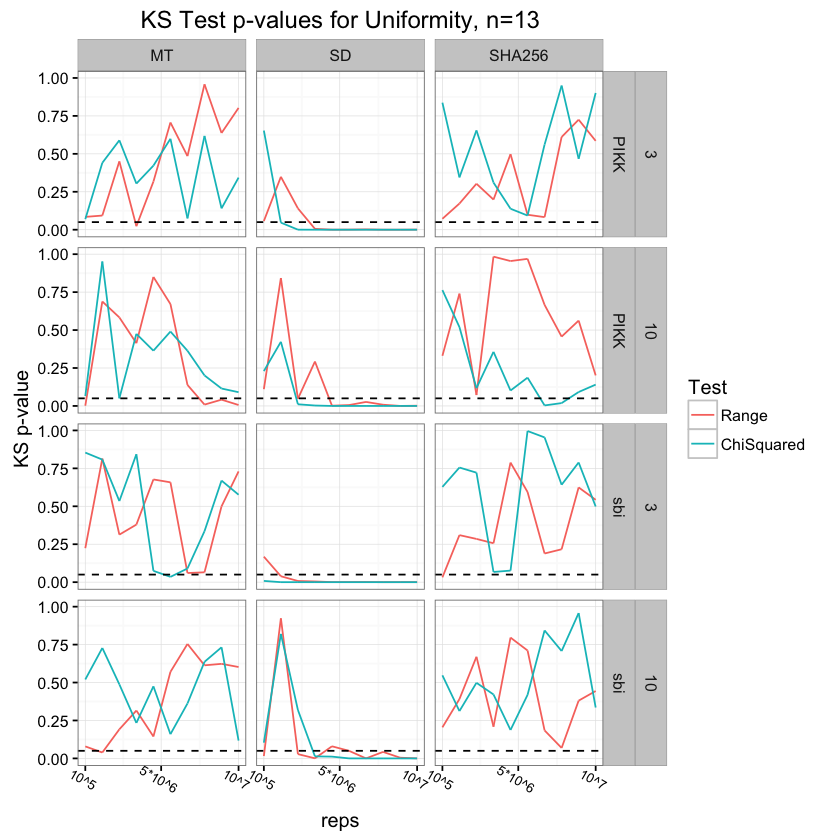
\includegraphics[width=0.8\textwidth]{fig/fixed-sample-size-ks-pvalues.png}
\caption{Kolmogorov-Smirnov test $p$-values for whether 1000 $p$-values appeared uniformly distributed. This figure displays these $p$-values for the chi-squared test and range statistic test of equiprobable multinomial categories, for varying sample sizes, number of replications, and sampling algorithms. PIKK abbreviates ``permute indices and pick $k$'' and sbi abbreviates ``sample by index''.}
\label{fig:fixed-sample-size}
\end{center}
\end{figure}

% Actual results are summarized in ``Code/frequencySimulations/results/thousandseedresults.ipynb''

\subsection{Sampling SPRT}
We used the SPRT to test whether these PRNGs produced simple random samples with uniform frequency.
We compared the same PRNGs and sampling algorithms as above
using a population of size $n=13$ and drew samples of size $k=3$. 
We specified the alternative probability of landing in one of the top $s$ categories as $p_1 = 1.01p_0$, to test the alternative hypothesis $p_1 > p_0$.
To test the lower-tailed alternative $p_1 < p_0$, we let $p_1 = 0.99 p_0$. 
Throughout, we varied the choice of $s$: 5, 10, 15, and 20. 
We used a type I error rate of $\alpha=0.025$ and type II error rate of $\beta = 0$; 
setting $\beta$ to zero ensures that we never accept the null hypothesis, but either reject it at level $\alpha$ or terminate after $10^6$ steps without making a decision.

Out of 1000 tests starting with different seeds, we rejected the null hypothesis less than $5\%$ of the time, for all of the PRNG and algorithm combinations. 
Figure~\ref{fig:multinomial_sprt_rejections} shows the rejection rates for the upper and lower tailed alternatives for each value of $s$: none exceeded $2.5\%$.
Differences in rejection rates between the PRNGs and sampling algorithms were not large or consistent.


\begin{figure}[h]
\begin{center}
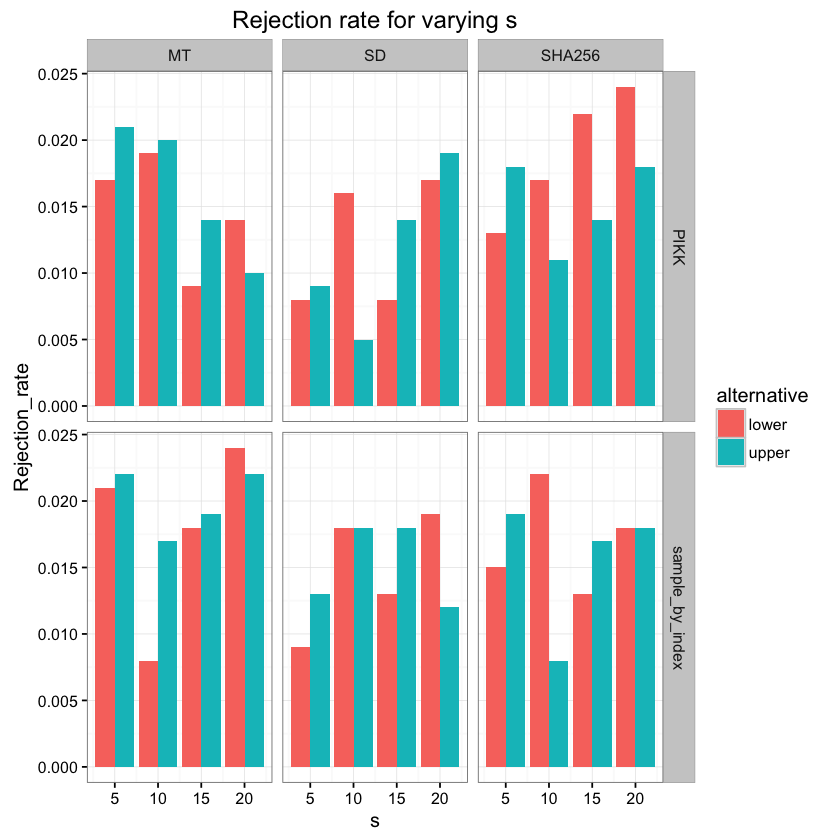
\includegraphics[width=0.8\textwidth]{fig/sprt-multinomial-rejection-rate.png}
\caption{Rejection rate of the multinomial SPRT for MT, SD, and SHA256, using the PIKK and sample by index algorithms to generate samples of size $3$ out of $13$. We varied $s$, a parameter of the test which specifies the number of ``most frequent'' or ``least frequent'' categories considered.  We rejected the null hypothesis less often than the specified type I error rate of $2.5\%$.}
\label{fig:multinomial_sprt_rejections}
\end{center}
\end{figure}

We subsetted to the tests which terminated with a decision to reject the null hypothesis of equal sample frequencies and compared the number of steps before termination for each PRNG and sampling algorithm combination. 
As $s$ increased, the number of steps needed to terminate the test decreased. 
This is expected, as increasing $s$ adds power. 
When pooling the upper- and lower-tailed test rejections, it is difficult to see any pattern in the number of steps needed to reject for the various PRNGs and sampling algorithms. 

When we separate upper- and lower-tailed rejections, some interesting patterns appear. 
In most cases, the lower alternative tended to be easier to reject (fewer steps) than the upper alternative for PIKK, suggesting that PIKK systematically generates certain samples with unusually low frequency. 
Conversely, in most cases the upper alternative tended to be easier to reject than the lower alternative for sampling by index, suggesting that this algorithm may favor certain samples.

\subsection{Derangement SPRT}
We used the SPRT to test whether derangements occur more or less often than expected due to chance alone.
We compared the three PRNGs above and used both the method of permuting indices and the FYKD shuffle to generate random permutations
of the list $(1, 2, \dots, n)$.
We increased $n$ from $500$ to $3000$ in increments of $500$.
The specified type I error rate was $2.5\%$ for the upper and lower alternatives.
We ran the test for 1000 different seeds for each PRNG and algorithm.

Figure~\ref{fig:derangement_sprt_rejections} shows the rejection rates for the upper and lower tailed alternatives for each value of $n$.
MT and SHA256 did not reject more often than expected under the null hypothesis
(for some of the experiments, the rejection rate is slightly higher than $2.5\%$ but it is within the expected margin of error of $\sqrt{0.025\times 0.975/1000} \approx 0.5\%$).
This was true for both sampling algorithms.
On the other hand, the Super-Duper LCG paired with the FYKD shuffle had rejection rates much higher than $2.5\%$ for $n\geq 1500$.
Both alternatives were rejected more often than $2.5\%$, but the upper-tailed alternative was rejected much more frequently.
This suggests that SD fails at producing permutations uniformly: depending on the seed, it may produce too many or too few
derangements compared with what a true random generator would produce.


\begin{figure}[h]
\begin{center}
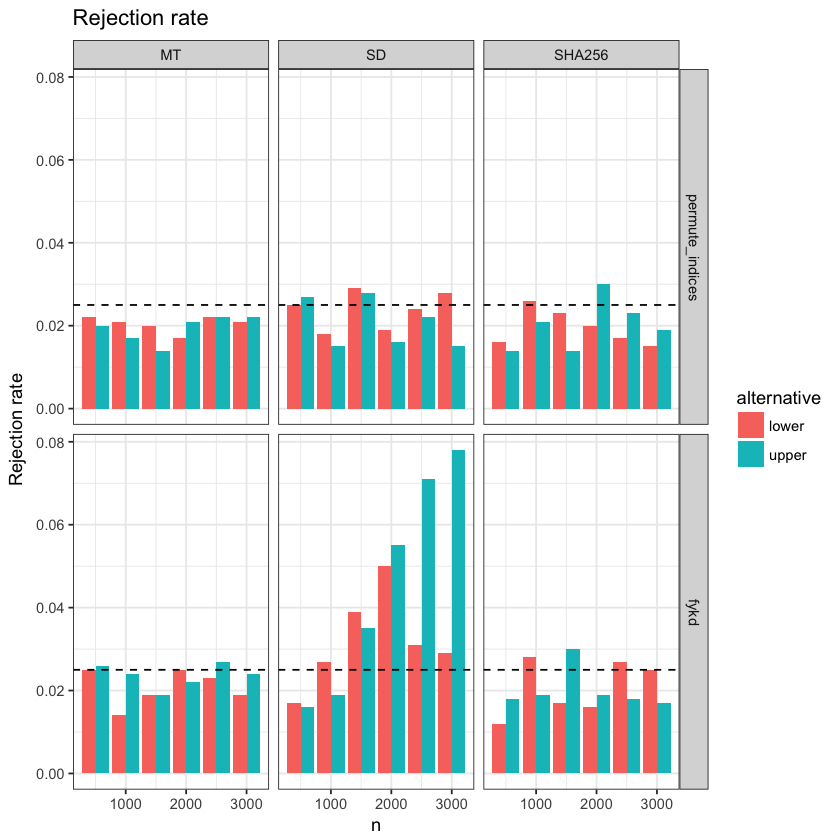
\includegraphics[width=0.8\textwidth]{fig/sprt-derangement-rejection-rate.png}
\caption{Rejection rate of the derangements SPRT for MT, SD, and SHA256, using the permute indices and FYKD shuffle algorithms to generate random permutations. We varied $n$, the length of the list being permuted.  The specified type I error rate was $2.5\%$ for the upper and lower alternatives.}
\label{fig:derangement_sprt_rejections}
\end{center}
\end{figure}

\subsection{Serial correlation test}
We generated $2 \times 10^5$ permutations of the numbers $(1, 2, \dots, N)$, for $N = 200, 500, 1000, $ and $2100$ 
and computed the distribution of the number of fixed points, then tested whether the observed distribution matched a Poisson distribution with parameter $1$.
Since the Poisson distribution is discrete and category probabilities quickly decrease to near zero, we conducted a chi-square test for goodness of fit with the observed distribution.
We used twelve categories for the chi-squared test: zero fixed points through ten fixed points, and a category for eleven or more fixed points.
In additional analyses, we varied the number of bins; the results were largely the same.

Neither MT nor the SHA256 PRNG showed evidence of departures from the expected distribution of fixed points between successive permutations for any value of $N$.
The distributions of chi-squared $p$-values were not significantly different from uniform.


\section{Discussion}\label{sec:discussion}



\todo{
Points to hit:
}

\begin{itemize}
\item These tests should be included in standard test batteries.
We developed the tests in Section~\ref{sec:tests} with the goal of checking a PRNG's fit for use in resampling statistics.
However, the ability to generate SRSs is also a measure of a good PRNG.
If a PRNG cannot hold up against one of the standing sampling algorithms, then is it really a good PRNG?

\item The speed of the SHA256 is prohibitive. 
Timing tests using our prototype implementation in Python indicate that it is twenty times slower than the Numpy Mersenne Twister to generate a single pseudorandom number, and nearly two hundred times slower than the Mersenne Twister for generating thousands of pseudorandom numbers.
Our first attempts to wrap C code with a Python interface slowed down the SHA256 PRNG by a factor of two.
For someone generating a single random sample or permutation from their data, then the one-time cost of using the SHA256 PRNG may be acceptable.
Work is needed to make the SHA256 PRNG efficient for resampling methods.

\item We have picked ``small'' (e.g. sampling 3 items out of 13) and ``medium'' sized problems (e.g. permuting 2000 items) and run them many times -- with thousands of replications and thousands of starting seeds.
We have not found evidence that Mersenne Twister fails to produce sufficiently random samples and permutations in these problems.
The extent to which we exercise the PRNGs for these problems is much more extensive than in real applications.
For instance, in social science applications, there are typically only hundreds of observations and one typically uses 1000 to 10,000 resamples in a permutation test.
If one runs many such tests, the number of PRNs they use remains within the scope of our tests.

\item Mersenne Twister may begin to fail these tests for ``large'' problems (e.g. population sizes in the millions).
Problems like this may arise in doing inference on data with a huge number of observations, 
such as data that websites that collect on their users,
or in fitting and doing inference on high-dimensional models, 
such as bootstrapping thousands of parameters.
We did not simulate scenarios like this due to computational constraints;
to run a large-scale procedure thousands of times would take weeks.
We believe it would be worthwhile to test a PRNG's fitness for use in these larger problems.

\item Table~\ref{tab:software} lists common software packages along with their default PRNG and algorithm for generating simple random samples. Discuss the implications of various algorithms across packages.
\end{itemize}


\begin{table}[h]
\caption{Key: MT = Mersenne Twister. LCG = linear congruential generator. The KISS generator combines 4 generators of three types: two multiply-with-carry generators, the 3-shift register SHR3 and the congruential generator CONG. }
\begin{center}
\begin{tabular}{l|c|c|c|}
Package/Lang & default & other & SRS algorithm \\
\hline
SAS 9.2 & MT & 32-bit LCG & Floyd's ordered hash table \\ % p 585 of SAS/STAT 9.3 User's Guide: Survey Data Analysis https://books.google.com/books?id=Rwi3m1QJro4C&pg=PA585&lpg=PA585&dq=Floyd?s+ordered+hash+table+algorithm+for+simple+random+sampling&source=bl&ots=BeorFtS0O-&sig=ngvFhIOxWLhBH_RJQtttIdTXPwg&hl=en&sa=X&ved=0ahUKEwj5n4SS9vDVAhULqFQKHXYUDMEQ6AEINTAC#v=onepage&q=simple%20random%20sample&f=false
SPSS 20.0 & 32-bit LCG & MT1997ar & truncate + random indices \\ % https://www.ibm.com/support/knowledgecenter/en/SSLVMB_20.0.0/com.ibm.spss.statistics.help/alg_csselect_systematic_algorithm.htm
SPSS $\leq$ 12.0 & 32-bit LCG & & \\
Stata 13 & KISS 32 & & PIKK \\
Stata 14 & MT & & PIKK \\
R & MT & & truncate + random indices \\
Python \texttt{random} & MT & & discard bits + random indices \\
Python \texttt{numpy} & MT & & discard bits + shuffle indices, keep $k$ \\
Matlab & MT & & truncate + PIKK
\end{tabular}
\end{center}
\label{tab:software}
\end{table}%



\subsection{Best Practices}

\todo{}

\bibliographystyle{plainnat}
\bibliography{refs}

\appendix


\section{Sampling algorithms}\label{sec:algorithms}
A simple random sample of size $k$ from a population of size $n$ is a sample drawn in such a way that each of the ${n \choose k}$ possible subsets of size $k$ is equally likely.
Given a good source of randomness, there are many ways to operationalize this definition to draw simple random samples.

\subsection{PIKK (permute indices and keep $k$)}
One basic approach is like shuffling a deck of $n$ cards, then dealing the top $k$: permute the population at random, then take the first $k$ elements of the permutation to be the sample.
There are a number of standard ways to generate a random permutation -- i.e., to shuffle the deck.
If we had a way to generate independent, identically distributed (iid) $U[0,1]$ random numbers\footnote{
Alternatively, one could generate independent and identically distributed random integers $1, \dots, n$.
What matters is not the range of values, but that numbers are uniformly distributed.}, we could sample $k$ out of $n$ as follows:

\begin{algorithm}                      % enter the algorithm environment
\caption{PIKK: Permute indices and keep $k$}          % give the algorithm a caption
\label{PIKK}                           % and a label for \ref{} commands later in the document
\begin{algorithmic}[1]               % enter the algorithmic environment
    \Require $n \geq k \geq 0$
    \Statex
     \State{Assign IID uniform values on $[0,1]$ to the $n$ elements of the population}
     \State{Sort the population according to these values (break ties randomly)}
     \State{Take the top $k$ to be the sample}
\end{algorithmic}
\end{algorithm}

This amounts to generating a random permutation of the population and throwing out all but the first $k$.
If the numbers really are independent and identically distributed, every permutation is equally likely, and it follows that the first $k$ are an SRS.
If permutations are not equiprobable, then samples generated using this algorithm may not be either.

Furthermore, this algorithm is inefficient: it requires the generation of $n$ random numbers and then an $O(n\log n)$ sorting operation.

\subsection{Shuffle}
There are more efficient ways to generate a random permutation than assigning a number to each element and sorting.
One example is the``Fisher-Yates shuffle'' or ``Knuth shuffle'' (Knuth attributes it to Durstenfeld).

\begin{algorithm}                      % enter the algorithm environment
\caption{Fisher-Yates-Knuth-Durstenfeld shuffle (backwards version)}          % give the algorithm a caption
\label{FYKD}                           % and a label for \ref{} commands later in the document
\begin{algorithmic}[1]               % enter the algorithmic environment
\For{$i = 1, \dots, n-1$}
    \Let{$J$}{random integer uniformly distributed on $i, \dots, n$}
    \Let{$(a[J], a[i])$}{$(a[i], a[J])$}
\EndFor
\end{algorithmic}
\end{algorithm}

This algorithm requires the ability to generate independent random integers on various ranges, but doesn't require sorting.
There is also a version suitable for streaming, i.e. generating a random permutation of a list that has an (initially) unknown number of elements.

\begin{algorithm}                      % enter the algorithm environment
\caption{Fisher-Yates-Knuth-Durstenfeld shuffle (streaming version)}          % give the algorithm a caption
\label{FYKD-streaming}                           % and a label for \ref{} commands later in the document
\begin{algorithmic}[1]               % enter the algorithmic environment
\Let{$i$}{0}
\Let{$a$}{[]}
\While{there are records left}
    \Let{$i$}{$i+1$}
    \Let{$J$}{random integer uniformly distributed on $\{1, \dots, i\}$}
    \If{$J < i$}
        \Let{$a[i]$}{$a[J]$}
        \Let{$a[J]$}{next record}
    \Else
        \Let{$a[i]$}{next record} 
    \EndIf
\EndWhile \\
\Return{$a$}
\end{algorithmic}
\end{algorithm}


\begin{proof}[Proof that the streaming shuffle works]
We prove by induction. The base case $i=1$ is trivial.
At stage $i$, $i>1$, suppose that all $(i-1)!$ permutations of $\{1, 2, \dots, i-1\}$ are equally likely.
$J$ may take on $i-1$ distinct values less than $i$, and the swapping procedure thus yields $(i-1)! \times (i-1)$
possible distinct permutations.
If $J = i$, then there is no swap and $(i-1)$ possible distinct permutations.
In total, there are $(i-1)! \times (i-1 + 1) = i!$ possible distinct permutations, and all are equally likely because
all values of $J$ and permutations of the first $(i-1)$ elements were equally likely.
\end{proof}


\subsection{\texttt{Random\_Sample}}
This algorithm is attributed to \citet{cormen_introduction_2009}.
It is a recursive algorithm that requires only $k$ random integers and does not require sorting.
\todo{prove by recursion that the method works}


\begin{algorithm}                      % enter the algorithm environment
\caption{$Random\_Sample$}
\label{Random_Sample}
\begin{algorithmic}[1]               % enter the algorithmic environment
\Require{$n \geq k \geq 0$}
\Statex
\Function{Random\_Sample}{$n, k$}
\If{$k$ is $0$}
    \Return{the empty set}
\Else
     \Let{$S$}{\texttt{Random\_Sample}($n-1, k-1$)}
     \Let{$i$}{random integer uniformly distributed on $\{1, \dots, n\}$} 
     \If{$i$ is in $S$}
           \Let{$S$}{$S \cup \{n\}$}
     \Else
            \Let{$S$}{$S\cup\{i\}$}  
     \EndIf, 
     \Return{$S$}
\EndIf
\EndFunction
\end{algorithmic}
\end{algorithm}

\section{Proofs}

\begin{proof}[Proof of Lemma~\ref{lemma:randint}]
Define $\tilde{X}$ to be a uniform random integer on $\{0, 1, \dots, 2^w - 1\}$.
The selection probability for a particular integer value is 

\begin{align*}
\pr\left(Y = y\right) &= \pr\left(1 + \lfloor mX \rfloor = y\right) \\
&= \pr\left(y-1 \leq mX < y\right) \\
&= \pr\left(\tilde{X} < \frac{y2^w}{m}\right) - \pr\left(\tilde{X} \leq \frac{(-1)y2^w}{m}\right)\\
&= \pr\left(\tilde{X} < \left\lfloor\frac{y2^w}{m}\right\rfloor\right) - \pr\left(\tilde{X} \leq \left\lfloor\frac{(y-1)2^w}{m}\right\rfloor\right)\\
&= 2^{-w}\left(k^+(y-1)- k^-(y-1)\right)
\end{align*}

\noindent where, for fixed $m$, we define $k^-(i) \equiv \min \{k: k2^{-w} \geq i/m\}$ for all $i$,
$k^+(i) \equiv \max \{k : k2^{-w} < i/m \} = k^-(i+1)-1$ for $i = 0, \dots, m-1$
and $k^+(m) \equiv 2^w$.
The maximum ratio of selection probabilities is 

\begin{align*}
\max_{i, j \in \{0, \ldots, m-1\}} \frac{k^+(i) - k^-(i)}{k^+(j) - k^-(j)}
&= \frac{ \max_{i=0}^{m-1} (k^+(i) - k^-(i))}{\min_{i=0}^{m-1} (k^+(i) - k^-(i))} \\
&= \frac{ \max_{i=0}^{m-1} (k^+(i) - k^+(i+1) + 1)}{\min_{i=0}^{m-1} (k^-(i+1) - k^-(i) - 1)} \\
&= \frac{\lceil 2^w/m \rceil + 1}{\lfloor 2^w/m \rfloor -1}.
\end{align*}
\end{proof}
\todo{is this proof right? seems wrong}


\begin{proof}[Proof of Lemma~\ref{lemma:l1bound}]
Fix $S \in \mathcal{S}$ and choose some $G \in \mathcal{G}$ such that $G(S) = 0$.
\begin{align*}
\lVert F - G \rVert_1 &= \sum_{\omega \in \Omega} \lvert F(\omega) - G(\omega) \rvert \\
&= \sum_{\omega \in S} \lvert F(\omega) - G(\omega) \rvert + \sum_{\omega \in S^c} \lvert F(\omega) - G(\omega) \rvert\\
&= \sum_{\omega \in S} \lvert F(\omega) \rvert + \sum_{\omega \in S^c} \lvert F(\omega) - G(\omega) \rvert\\
&= \frac{ \lvert S \rvert}{{n \choose k}}+ \sum_{\omega \in S^c} \lvert F(\omega) - G(\omega) \rvert\\
&\geq \frac{ \lvert S \rvert}{{n \choose k}}+ \left\lvert\sum_{\omega \in S^c} \left( F(\omega) - G(\omega) \right)\right\rvert\\
&= \frac{ \lvert S \rvert}{{n \choose k}}+ \left\lvert\sum_{\omega \in S^c} F(\omega) - 1 \right\rvert\\
&= \frac{2 \lvert S \rvert}{{n \choose k}}
\end{align*}

Finally, $ \lVert F - G \rVert_1 \geq \inf_{S \in \mathcal{S}} \frac{2 \lvert S \rvert}{{n \choose k}} \geq \frac{2\nu}{{n \choose k}}$.
\end{proof}

%\begin{proof}[another way]
%Fix $S$ and choose $G \in \mathcal{G}$ such that $G(S) = 0, G(\omega) > 0$ for $\omega \in S^c$.
%\begin{align*}
%\lVert F - G \rVert_1 &= \sum_{\omega \in \Omega} \lvert F(\omega) - G(\omega) \rvert \\
%&= \sum_{\omega \in S} \lvert F(\omega) - G(\omega) \rvert + \sum_{\omega \in S^c} \lvert F(\omega) - G(\omega) \rvert\\
%&= \sum_{\omega \in S} \lvert F(\omega) \rvert + \sum_{\omega \in S^c} \lvert F(\omega) - G(\omega) \rvert\\
%&= \frac{ \lvert S \rvert}{{n \choose k}}+ \sum_{\omega \in S^c} \lvert F(\omega) - (F(\omega) + \eps_\omega) \rvert\\
%\end{align*}
%
%\noindent where $\eps_\omega \in [ - {n \choose k}^{-1}, 1 - {n\choose k}^{-1}]$ and $\sum_{\omega \in S^c} \eps_\omega = \sum_{\omega \in S} F(\omega) =  \frac{ \lvert S \rvert}{{n \choose k}}$.
%NB this must be the case to ensure that $\sum_{\omega} G(\omega) = 1$, since
%$$\sum_{\omega} G(\omega) =\sum_{\omega\in S^c} G(\omega) = \sum_{\omega\in S^c} F(\omega) + \eps_\omega = \sum_{\omega\in S^c} F(\omega) + \sum_{\omega\in S} F(\omega) = 1.$$
%
%Therefore,
%\begin{align*}
%\lVert F - G \rVert_1 &= \frac{ \lvert S \rvert}{{n \choose k}}+ \sum_{\omega \in S^c} \lvert \eps_\omega \rvert\\
%&=  \frac{ \lvert S \rvert}{{n \choose k}}+ \sum_{\omega \in S} \lvert F(\omega) \rvert \\
%&= \frac{2 \lvert S \rvert}{{n \choose k}}
%\end{align*}
%\end{proof}



\begin{theorem}\label{thm:poisson_approx}
The distribution of the number of points fixed between two random permutations is asymptotically Poisson distributed with parameter $1$.
For any list length $n$,

$$\lvert \mathbb{P}(S_n = k)-\mathbb{P}(W = k)\rvert \leq \frac{1}{k!}\frac{1}{(n-k+1)!}.$$
Furthermore, using the Poisson approximation instead of the exact distribution to compute expected cell counts for the chi-squared statistic inflates the chi-squared statistic by a factor of at most $n^{-2n}$.


\end{theorem}

\begin{proof}


Let $S_n$ denote the number of matches between the previous permutation and the current permutation.
As before, $D_n$ denotes the number of derangements of $n$ items.
$D_n$ satisfies the recurrence relation $D_n = (n-1)\left( D_{n-1} + D_{n-2}\right)$ with initial values $D_1 = 0, D_2 = 1$.

\begin{align*}
P(S_n=0) &= \frac{D_n}{n!} \\ 
P(S_n=1) &= \frac{n D_{n-1}}{n!} \\
\vdots \\
P(S_n = k) &= \frac{{n \choose k} D_{n-k}}{n!} 
\end{align*}

The number of matches $S_n$ is a sum of indicator variables, one for each position in the list. $X_i = 1$ if position $i$ is the same in the two permutations and $0$ otherwise. 
The probability that position $i$ is fixed is $\frac{1}{n}$, for each $i$.

The sum of correlated Bernoulli random variables is asymptotically Poisson distributed, with parameter equal to the sum of all of the Bernoulli parameters. 
We'll show that $S_n$ can be approximated well by a Poisson random variable with parameter $1$.
We begin by writing explicitly the probability distribution of $S_n$.

\begin{align*}
\mathbb{P}(S_n = k) &= \frac{{n \choose k} D_{n-k}}{n!} \\
&= \frac{n! D_{n-k}}{n! (n-k)! k!} \\
&= \frac{!(n-k)}{(n-k)!k!} \\
&= \frac{(n-k)! \sum_{i=0}^{n-k}\frac{(-1)^i}{i!}}{(n-k)!k!} \\
&= \frac{1}{k!} \left( \sum_{i=0}^{n-k} \frac{(-1)^i}{i!} \right)
\end{align*}

Let $W$ be a Poisson(1) random variable, so $\mathbb{P}(W=k) = \frac{e^{-1}}{k!}$.
For any $k\geq0$, the approximation error is 

$$\lvert \mathbb{P}(S_n = k)-\mathbb{P}(W = k)\rvert = \Big\lvert \frac{1}{k!} \sum_{i=n-k+1}^{\infty} \frac{(-1)^i}{i!} \Big\rvert \leq \frac{1}{k!}\frac{1}{(n-k+1)!} $$


Now, we are interested in how this approximation error shows up in the chi-squared test.
We'll consider the $k$th component of the chi-squared statistic.
When we use the approximate distribution, there is some error $\delta$ in computing the expected number in category $k$.
To first order,

\begin{align*}
\frac{(O_k-E_k-\delta)^2}{E_i+\delta} &= \frac{(O_i-E_i)^2}{E_i} + \delta\left( 1- \frac{O_i^2}{E_i^2}\right) \\
&= \frac{(O_i-E_i)^2}{E_i}\left( 1 + \frac{\delta}{E_i} \right) 
\end{align*}

Above, we found that $\delta \leq \frac{\text{reps}}{k!(n-k+1)!}$ and $E_k = \frac{\text{reps}}{k!}\sum_{j=0}^{n-k}\frac{(-1)^j}{j!} = \frac{\text{reps}}{k!} \left(e^{-1} - \delta k!\right)$.

$$ \frac{\delta}{E_k} \leq \frac{1}{(n-k+1)! (e^{-1} - \frac{1}{(n-k+1!)})} \approx \frac{1}{n^{2n}}.$$

Thus, the chi-squared statistic is inflated by a factor of at most $n^{-2n}$.
This becomes miniscule as $n$ increases.

\end{proof}

\end{document}
